% Synthetic fixture: a miniature structural diagram through the node-shape
% subset — circle and rectangle outlines with draw/fill/dashed/thick and
% declared minimums, style bundles, math node bodies, transform shape.
% Invented content and design.
\documentclass{article}

\fonts{ dir = "fonts", body = "Source Serif Pro" }

\begin{document}

\section{Shaped nodes}

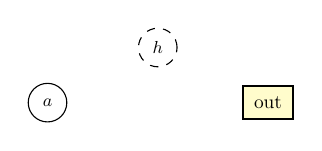
\begin{tikzpicture}[
  scale=0.7, transform shape,
  ball/.style={circle, draw, minimum size=7mm, inner sep=1pt, font=\small},
  hidden/.style={circle, draw, dashed, minimum size=7mm, font=\small},
  slab/.style={rectangle, draw, thick, fill=yellow!20, minimum width=9mm, minimum height=6mm}
]
  \node[ball]   (a) at (0, 0) {$a$};
  \node[hidden] (h) at (2, 1) {$h$};
  \node[slab]   (o) at (4, 0) {out};
\end{tikzpicture}

\end{document}
